\documentclass[twoside,11pt]{article}
\usepackage{jmlr2e}
\usepackage{graphicx}
\graphicspath{ {./images/} }
\usepackage{enumitem}
\newlist{mylistenv}{enumerate}{3}
\newenvironment{mylist}[1]{%
	\setlist[mylistenv]{label=#1\arabic{mylistenvi}.,ref=#1\arabic{mylistenvi}}%
	\setlist[mylistenv,2]{label=#1\arabic{mylistenvi}.\arabic{mylistenvii}.,ref=#1\arabic{mylistenvi}.\arabic{mylistenvii}}%
	\setlist[mylistenv,3]{label=#1\arabic{mylistenvi}.\arabic{mylistenvii}.\arabic{mylistenviii}.,ref=#1\arabic{mylistenvi}.\arabic{mylistenvii}.\arabic{mylistenviii}}%
	\renewenvironment{mylist}{\begin{mylistenv}}{\end{mylistenv}}
	\begin{mylistenv}%
	}{%
	\end{mylistenv}%
}
\newcommand\tab[1][1cm]{\hspace*{#1}}

% Definitions of handy macros can go here

\newcommand{\dataset}{{\cal D}}
\newcommand{\fracpartial}[2]{\frac{\partial #1}{\partial  #2}}


\firstpageno{1}

\begin{document}

\title{Project 5: Reinforcement Learning}

\author{\name Sarah Wilson 
	   \email swi1s117@jhu.edu \\
	   \phone 303-921-7225 \\
       \addr Engineering Professionals Computer Science\\
       Johns Hopkins University\\
       Baltimore, MD 21218, USA} 

\maketitle


\section{Introduction}
\hspace*{10mm} Reinforcement Learning (RL) is an area of Machine Learning that uses experiences to determine the next optimal decision. Typical the reinforcement learning process can be broken down into a few key steps: Observe the environment, decide how to act based on a policy, act based on that policy, be rewarded or penalized for that action, update the policy, iterate until the best policy is produced. Two major type of RL algorithms are the model-based and model-free algorithms. In the model-based algorithms a the function used to issue the reward is used to determine the best policy. In model-free algorithms, the reward function or the environmental updates are not used to determine the best policy. An example of a model-free algorithm is the Q-Learning algorithm. In Q-Learning, it is considered an off policy learner, because it learns the policy without needing to know the agent's actions. INSERT MORE ABOUT Value, Q and SARSA. \\



\hspace*{10mm} The objective of this paper is to explore three different reinforcement learning algorithms, Value Iteration, Quality Learning or Q-Learning and the State Action Reward State Action (SARSA) algorithm. These algorithms will be explored and implemented through the racetrack problem. In the racetrack problem, the objective is to get a car from the starting line to the finish line in as little time as possible. The racetrack will be described as a two dimensional Cartesian plane, where the location of the car on the racetrack can be described as a point pair $(x,y)$. The active control exerted over the car will be acceleration $a_x$ and $a_y$. The range of values that can be assigned to $a_x$ and $a_y$ are -1,0,1. The velocity of the car will be capped to values between -5 and 5, any acceleration values that cause the velocity to go beyond these bounds will be ignored. Additional the probability of the acceleration control being applied on each time step is 80\%, meaning there is a 20\% chance the accelerate control is issued no acceleration updates will occur. The experiments for these algorithms will occur on three uniquely shaped racetracks, the R-Shaped, O-Shaped and L-Shaped tracks.\\ 
\hspace*{10mm} An additional constraint that will be applied to this problem, is the consequence of a crash. A crash is defined as the car intersecting with the walls of the racetrack, in one variation if a crash happens, the car will be placed back to a location on the track nearest to the crash site with a zero velocity component. In the second, harsher variation, if a crash happens, the car will be placed back at the start of the racetrack with a zero velocity component. These variations will only be applied to the R-Shaped race track, the O-Shaped and L-Shaped tracks will not implement the harsher variation of the crash, instead if a crash occurs on these tracks the car will be placed at a location nearest to the crash site. \\
\hspace*{10mm} The hypothesis presented in this paper predicts that the SARSA algorithm will perform better compared to the Q-Learning or Value Iteration algorithms. The reason for this hypothesis is that the SARSA algorithm is an on-policy algorithm as it updates the policy based on the current choices of the policy that is being implemented. The Q-Learning algorithm, however, does not update the same policy used to explore the world. The SARSA algorithm seems better suited for the racetrack problem, since the actions taken by the model to drive the car the fastest around the racetrack should update the policy as the world is better understood, if the model understand there is a wall or turn coming up, it will have the environment baked into the policy, where as the Q-Learning or Value Iteration algorithms, do not account for updates to the environment each time the policy is updated.\\ 
\hspace*{10mm} Section 1 has provided the introduction, problem statement and hypothesis in regards to three major learning algorithms that will be explored. Section 2 will provide an in-depth explanation of the algorithms. Section 4 will present the results obtained by the different algorithms. Section 5 will discuss the results that were obtained and compare them to the hypothesis that was outlined in the introduction. This report will conclude in Section 6 with a discussion of lessons learned and areas of possible future work.\\


\section{Algorithms and Experimental Methods}
\textbf{Value Iteration}
\newpage

\textbf{Q-Learning}
\newpage

\textbf{SARSA}
\newpage


\section{Data Sets}
\hspace*{10mm} For this paper there were no explicate data-sets provided. Instead the data provided was in the form of the shape of the Racetracks. There were three uniquely shaped racetracks, the R-Shaped, O-Shaped and L-Shaped tracks provided for this problem. Each taking on the shape of the letter in their respective names.\\
	
\section{Results}
\hspace*{10mm} Tables 1-2 display the results from the R-Shaped race track across the three major algorithms. Table 1 details the results obtained when the crash variation was set to the instance where a crash occurs, the car is placed in a location nearest to the crash. Table 2 details the results obtained from the harsher variation of the crash, where the car is placed back at the starting line when a crash occurs. Table 3 and 4 display the results obtained from the O-Shaped and L-Shaped race tracks across the three major algorithms.\newline

\begin{table}[h]
		\centering
		\caption{R-Shaped Racetrack: Reinforcement Learning - Experimental Results\\ Crash Variation 1}
		\label{tab:table1}
		%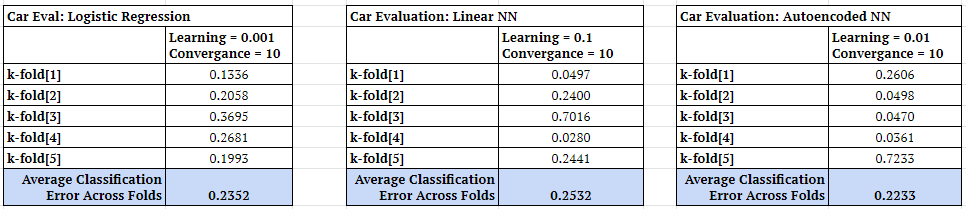
\includegraphics[scale=.7]{CarEval_All_Results}\newline
\end{table}

\begin{table}[h]
	\centering
	\caption{R-Shaped Racetrack: Reinforcement Learning - Experimental Results\\ Crash Variation 2}
	\label{tab:table2}
	%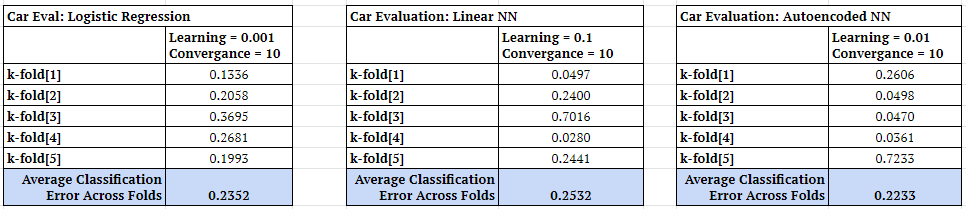
\includegraphics[scale=.7]{CarEval_All_Results}\newline
\end{table}

\begin{table}[h]
	\centering
	\caption{O-Shaped Racetrack: Reinforcement Learning - Experimental Results}
	\label{tab:table3}
	%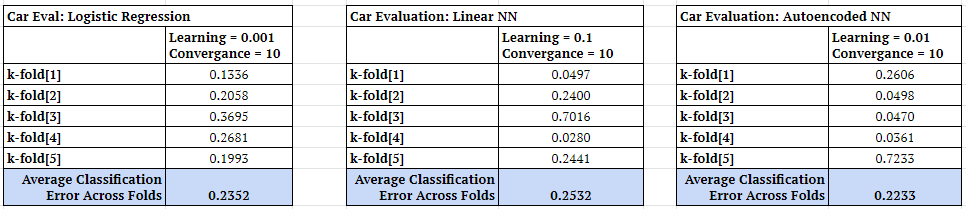
\includegraphics[scale=.7]{CarEval_All_Results}\newline
\end{table}

\begin{table}[h]
	\centering
	\caption{L-Shaped Racetrack: Reinforcement Learning - Experimental Results}
	\label{tab:table4}
	%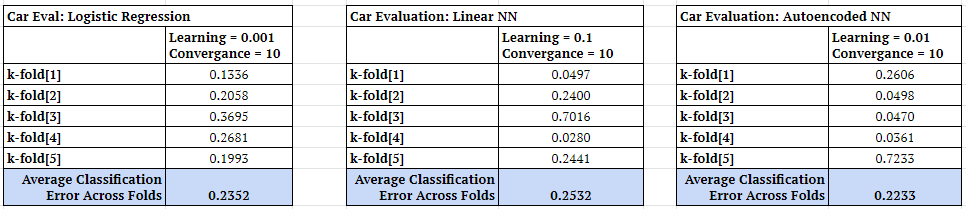
\includegraphics[scale=.7]{CarEval_All_Results}\newline
\end{table}

\newpage

\section{Discussion}
\hspace*{10mm} The hypothesis presented in this report was that the SARSA algorithm will perform better compared to the Q-Learning or Value Iteration algorithms.\\

\section{Conclusion}
\hspace*{10mm} Overall.\newline
\hspace*{10mm} A suggested area of future work, INSERT\newline

\section{References}
1. Alpaydin, E. (2004). Introduction to machine learning (Oip). Mit Press. 

\newpage


\end{document}